\begin{frame}
	\frametitle{Aufgabe 1) Evaluate}
	\framesubtitle{Aufgabenstellung und Problem}
	\setbeamertemplate{enumerate items}[default]
	ABS-Normal Form:
	\begin{flalign*}
		\begin{pmatrix}
		\Delta z \\
		\Delta y
		\end{pmatrix}
		= 
		\begin{pmatrix}
		a \\
		b
		\end{pmatrix}
		+
		\begin{pmatrix}
		Z & L \\
		J & Y 
		\end{pmatrix}
		\times
		\begin{pmatrix}
		\Delta x \\
		|\Delta z |
		\end{pmatrix}
	\end{flalign*}
	Gegeben:
	\begin{flalign*}
		a,b,Z,L,J,Y,m,n,s, \Delta x
	\end{flalign*}
	Gesucht:
	\begin{flalign*}
		\Delta z, \Delta y
	\end{flalign*}
	\begin{flalign*}
		\Delta y &= b + (J \times \Delta x) + (Y \times |\Delta z|) \\
		\Delta z &= a + (J \times \Delta x) + (L \times |\Delta z|)
	\end{flalign*}
	Problem:
	\begin{flalign*}
		\highlightred{\Delta z} &= a + (J \times \Delta x) + (L \times\highlightred{ |\Delta z|})
	\end{flalign*}
\end{frame}
%----------------------------------------------------------------------------
\begin{frame}
\frametitle{Aufgabe 1) Evaluate}
\framesubtitle{Löse $z = f(|\Delta z|)$}
\setbeamertemplate{enumerate items}[default]

	
\begin{flalign*}
	\left(\begin{array}{c}
	\Delta z_1 \\
	\Delta z_2 \\
	\Delta z_3 \\
	\Delta z_4 \\
	\end{array}\right) = 
	\left(\begin{array}{c}
	k_1 \\
	k_2 \\
	k_3 \\
	k_4 \\
	\end{array}\right) +
	\left(\begin{array}{cccc}
	0 		& 0 	  & 0  & 0 \\
	L_{2,1} & 0 	  & 0  & 0 \\
	L_{3,1} & L_{3,2} & 0  & 0\\
	L_{4,1} & L_{4,2} & L_{4,3} & 0 \\
	\end{array}\right) \times
	\left(\begin{array}{c}
	|\Delta z_1 | \\
	|\Delta z_2 | \\
	|\Delta z_3 | \\
	|\Delta z_4 | \\
	\end{array}\right)
\end{flalign*}
\begin{flalign*}
	k = a + Z \times \Delta x
\end{flalign*}

\begin{flalign*}
	\highlightblue{\Delta  z_1}  &= \underbrace{L_1 \times |\Delta z|}_{=0} + k_1 = k_1 \\
	\highlightyellow{\Delta z_2} &= L_2 \times |\Delta z| + k_2 \\
								 &= L_{2,1} \times \highlightblue{|\Delta z_1 |} + k_2 \\
		\highlightgreen{\Delta z_3} &= L_3 \times |\Delta z| + k_3 \\
		&= L_{3,1} \times \highlightblue{|\Delta z_1 |} + L_{3,2} \times \highlightyellow{|\Delta z_2|} + k_3 \\
		\highlightred{\Delta z_4} &= L_{4} \times |\Delta z| + k_4 \\
		&= L_{4,1} \times \highlightblue{|\Delta z_1|} + 
		L_{4,2} \times \highlightyellow{|\Delta z_2|} +
		L_{4,3} \times \highlightgreen{|\Delta z_3|} + k_4 \\
\end{flalign*}
\end{frame}
%----------------------------------------------------------------------------
\begin{frame}[fragile]
	\frametitle{Aufgabe 1) Evaluate}
	\framesubtitle{Implementierung}
	\begin{lstlisting}[language=cpp]
	template <typename T>
	void eval(T *a, T *b, 
			  T *Z, T *L, 
			  T *J, T *Y,
			  T *dx,
			  int m, int n, int s,
			  T *dz, T *dy,
			  T *abs_dz)
	{
			// dz = a
			cudaMemcpy(dz, a, ., cudaMemcpyDeviceToDevice));
			// dz = Z * dx + dx
			cublasDgemv(.,Z, ., dx, . dz, .)
			// dz[i] = L[i]_i * |dz|_i
			for(int i=0; i<s; i++)
			{
				cublasDgemv( . ,&L[i * s], . ,abs_dz, . , &dz[i],.);
				abs <<<1,1>>>(&dz[i], &abs_dz[i], 1);
			}
			// dy = b
			cudaMemcpy(dy, b, ., cudaMemcpyDeviceToDevice);
			// dy = dy + J*dx
			cublasDgemv(.,J, ., dx, ., dy, .));
			// dy = dy + Y * |dz|
			cublasDgemv(., Y, ., abs_dz, ., dy, .));
	}
	\end{lstlisting}
\end{frame}
%----------------------------------------------------------------------------
\begin{frame}
	\frametitle{Aufgabe 1) Evaluate}
	\framesubtitle{Speicherkomplexität}
	\setbeamertemplate{enumerate items}[default]
	Speicherkomplexität: \\
	\begin{center}
		\begin{tabular}{ c | c | c | c | c | c | c | c | c | c }
		$a$ & $b$ & $Z$ & $L$ & $J$ & $Y$ & $\Delta y$ & $\Delta x$ & $\Delta z$ & $|\Delta z|$\\
		\hline
		$s$ & $m$ & $s*n$ & $s*s$ & $m*n$ & $m*s$ & $m$ & $n$ & $s$& $s$\\
		\end{tabular}
	\end{center}
	\begin{flalign*}
		(s^2 + (3 + m + n)*s + (m + 2)m + n) * sizeof(T)
	\end{flalign*}
	Seien 
	\begin{itemize}
		\item $m = 1000, n = 1000, s=1000$
		\item Datatype: $double \approx 8 bytes$
		\item $32.048.000$ Bytes $\approx 0.032048 GB$
	\end{itemize}
	Seien 
	\begin{itemize}
		\item $m = 1000, n = 1000, s=100.000$
		\item Datatype: $double \approx 8 bytes$
		\item $81.610.424.000$ Bytes $\approx 81.610 GB$
		\end{itemize}
\end{frame}
%----------------------------------------------------------------------------
\begin{frame}
	\frametitle{Aufgabe 1) Evaluate}
	\framesubtitle{Komplexität}
	\setbeamertemplate{enumerate items}[default]
	Komplexität:
	\begin{center}
	\begin{tabular}{ l | c | c}
		Funktion & Komplexität Seriell & Komplexität Parallel \\
		\hline
		$cudaMemcpy(dz,a)$	& $s$ & $s/p$  \\
		$cublasDgemv(Z,dx,dz)$& $s*n$ & $(s*n)/p$ \\
		$cublasDgemv(L, |dz|)$& $s*s$ & $(s*s)/p$ \\
		$cublasMemcpy(dy,b)$  & $m$  & $m/p$ \\
		$cublasDgemv(J,dx,dy)$& $m*n$ & $(m*n)/p$ \\
		$cublasDgemv(Y, |dz|, dy)$ & $m*s$ & $(m*s)/p$ \\
	\end{tabular} 	\\~\\
	\end{center}
	
	Der Rechenaufwand steigt im selben Maße wie der Speicheraufwand ! \\
	
	\begin{center}
		Vermutung, parallelisieren bringt hier nicht viel!
	\end{center}
	Flaschenhals: Speicher, Speicheroperationen
\end{frame}
%----------------------------------------------------------------------------
\setbeamertemplate{navigation symbols}{}
\begin{frame}[plain]
	\makebox[\linewidth]{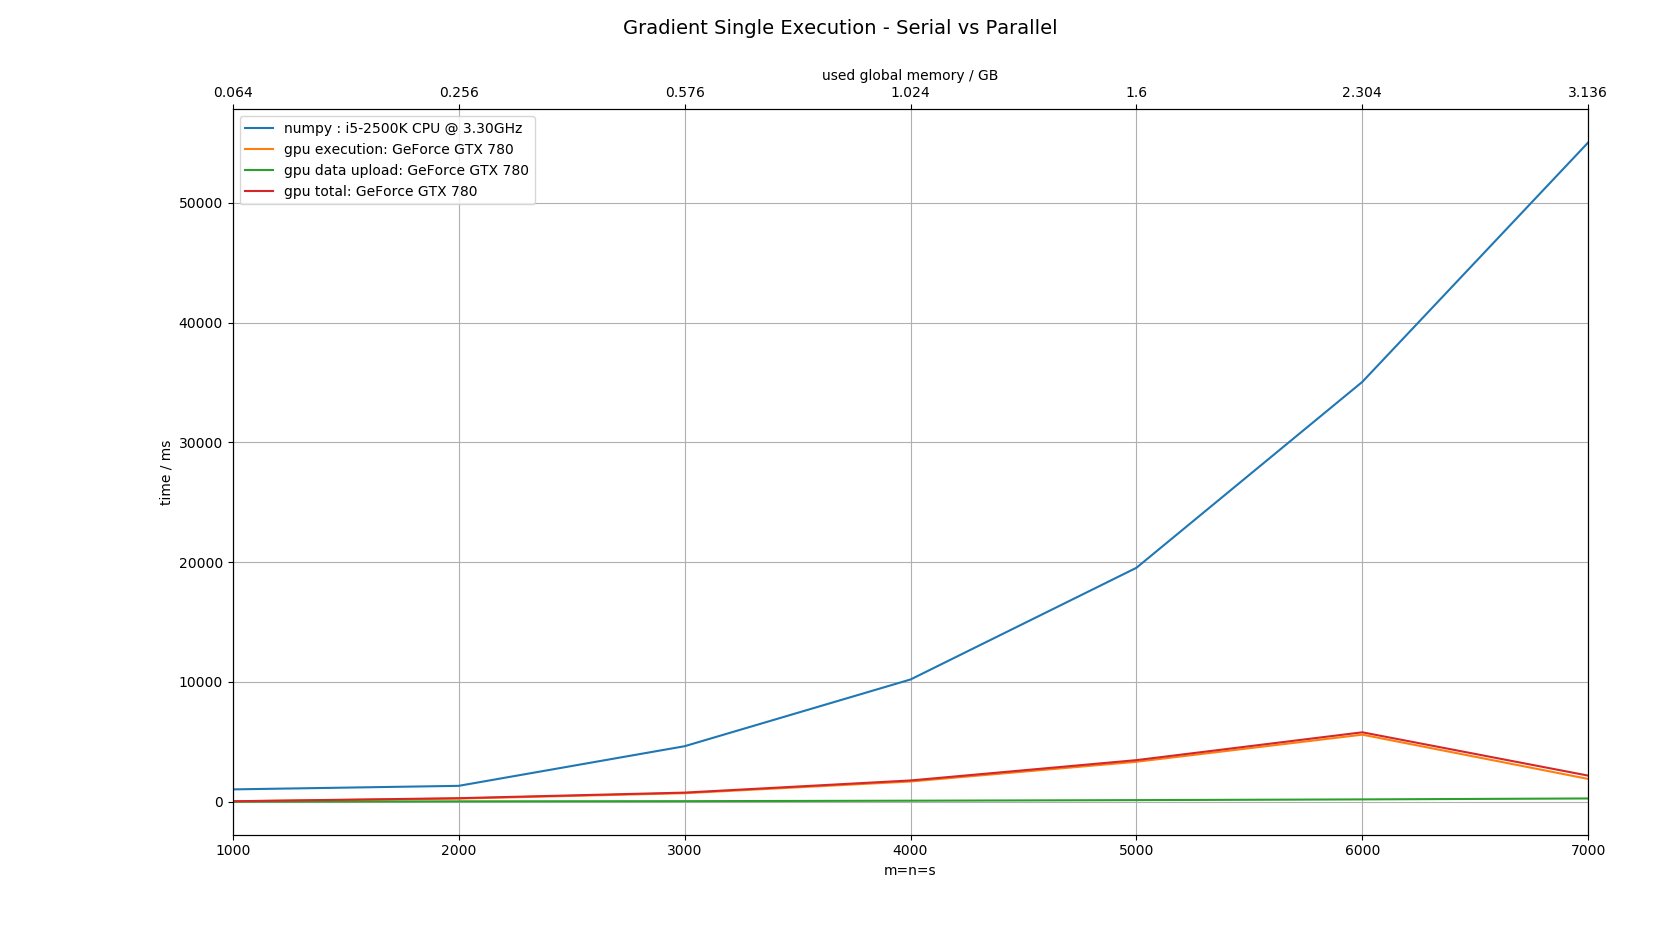
\includegraphics[width=\paperwidth]{img/eval-single.png}}
\end{frame}
%----------------------------------------------------------------------------
\setbeamertemplate{navigation symbols}{}
\begin{frame}[plain]
	\makebox[\linewidth]{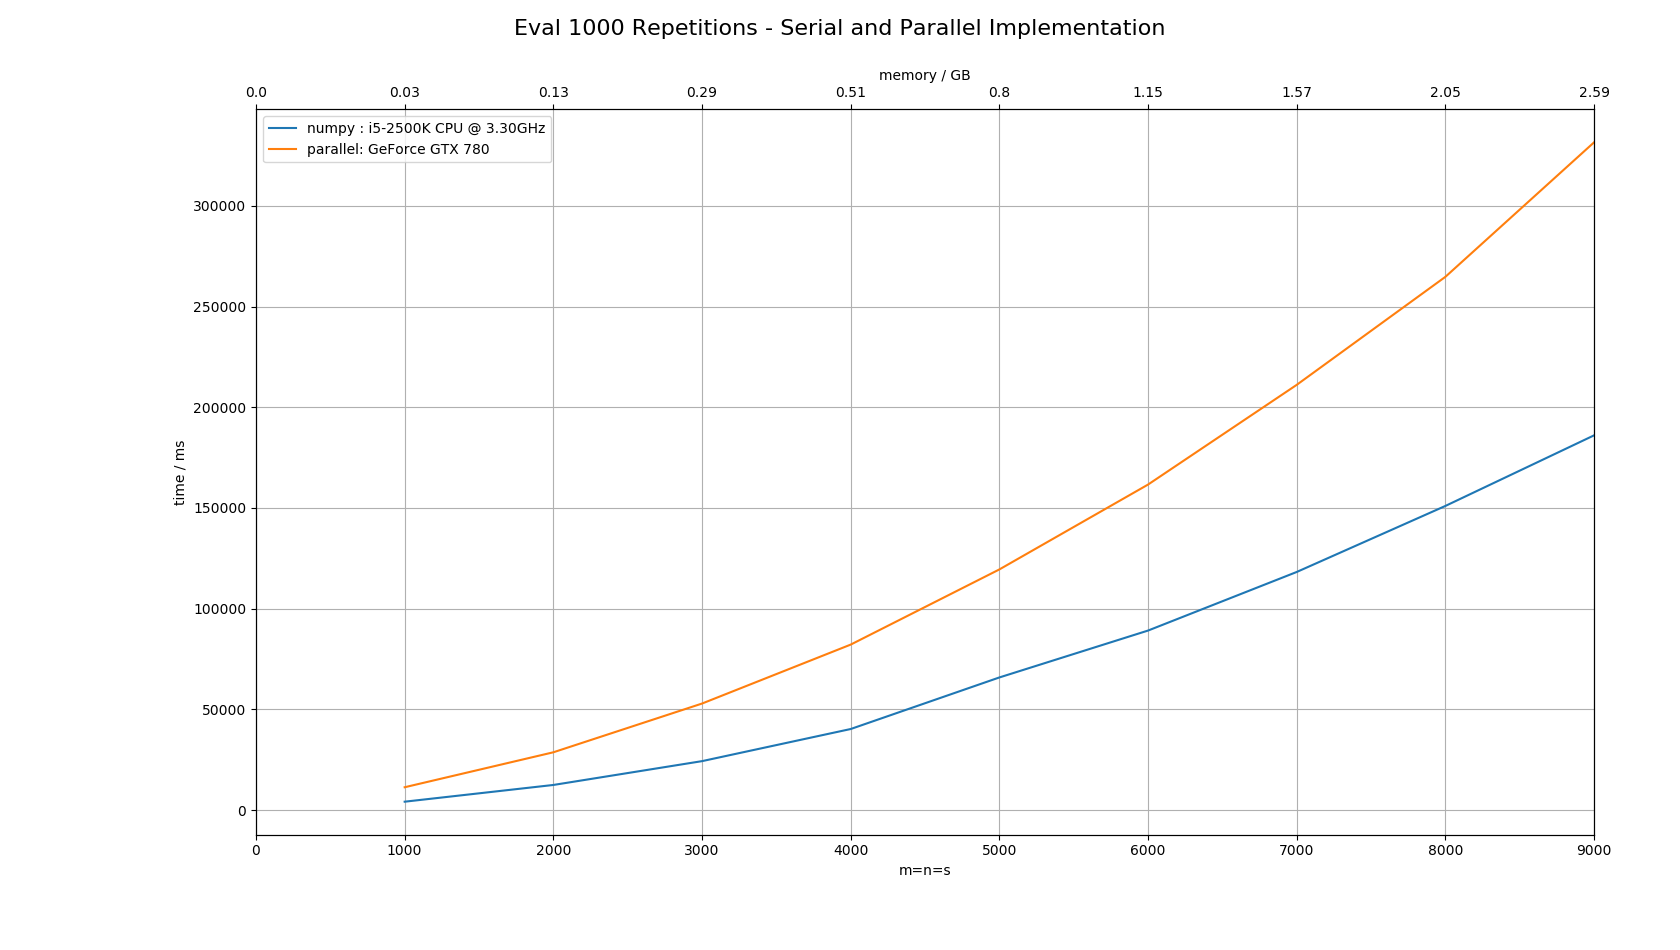
\includegraphics[width=\paperwidth]{img/eval-100.png}}
\end{frame}